\begin{minipage}{0.75\linewidth}
\begin{figure}[h]
    \centering
    \begin{adjustbox}{max width=1.0\linewidth, keepaspectratio}
        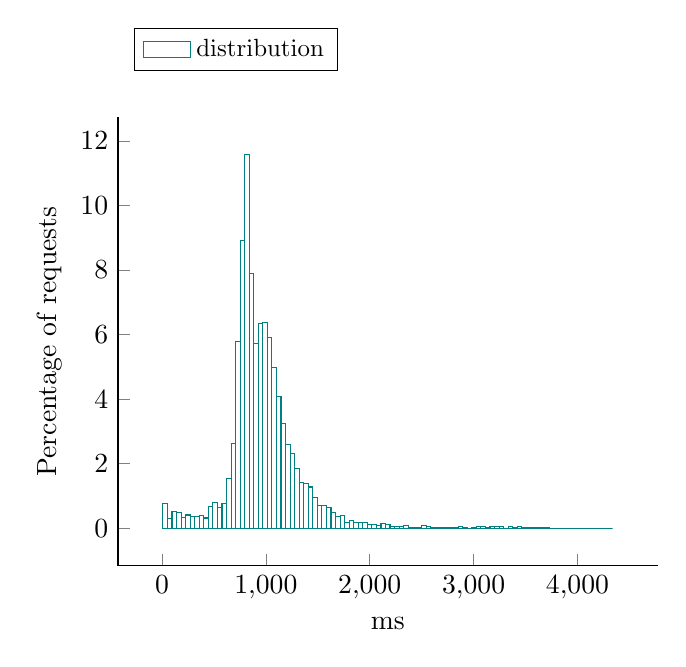
\begin{tikzpicture}
            \begin{axis}[ylabel = Percentage of requests, 
xlabel = ms, 
legend style = {nodes={scale=0.9, transform shape}, at={(0.03,1.2)}, anchor=north west, draw=black, fill=white, align=left, legend columns=3},
area style, mark size = 0pt,
 cycle list name = exotic,
  axis lines* = left]
		\addplot +[ybar interval] coordinates {
			 (9, 0.761421)
			 (52.73, 0.296108)
			 (96.46, 0.507614)
			 (140.19, 0.497039)
			 (183.92, 0.338409)
			 (227.65, 0.412437)
			 (271.38, 0.35956)
			 (315.11, 0.370135)
			 (358.84, 0.401861)
			 (402.57, 0.317259)
			 (446.3, 0.666244)
			 (490.03, 0.803723)
			 (533.76, 0.645093)
			 (577.49, 0.771997)
			 (621.22, 1.53342)
			 (664.95, 2.6121)
			 (708.68, 5.79526)
			 (752.41, 8.92555)
			 (796.14, 11.5694)
			 (839.87, 7.89975)
			 (883.6, 5.73181)
			 (927.33, 6.34518)
			 (971.06, 6.36633)
			 (1014.79, 5.91159)
			 (1058.52, 4.98096)
			 (1102.25, 4.08206)
			 (1145.98, 3.23604)
			 (1189.71, 2.59095)
			 (1233.44, 2.32657)
			 (1277.17, 1.85068)
			 (1320.9, 1.40651)
			 (1364.63, 1.38536)
			 (1408.36, 1.27961)
			 (1452.09, 0.962352)
			 (1495.82, 0.708545)
			 (1539.55, 0.708545)
			 (1583.28, 0.645093)
			 (1627.01, 0.497039)
			 (1670.74, 0.370135)
			 (1714.47, 0.401861)
			 (1758.2, 0.17978)
			 (1801.93, 0.232657)
			 (1845.66, 0.190355)
			 (1889.39, 0.17978)
			 (1933.12, 0.169205)
			 (1976.85, 0.105753)
			 (2020.58, 0.126904)
			 (2064.31, 0.0951777)
			 (2108.04, 0.137479)
			 (2151.77, 0.126904)
			 (2195.5, 0.0634518)
			 (2239.23, 0.0634518)
			 (2282.96, 0.0634518)
			 (2326.69, 0.0846024)
			 (2370.42, 0.0105753)
			 (2414.15, 0.0317259)
			 (2457.88, 0.0211506)
			 (2501.61, 0.0740271)
			 (2545.34, 0.0634518)
			 (2589.07, 0.0317259)
			 (2632.8, 0.0105753)
			 (2676.53, 0.0211506)
			 (2720.26, 0.0105753)
			 (2763.99, 0.0105753)
			 (2807.72, 0.0211506)
			 (2851.45, 0.0423012)
			 (2895.18, 0.0211506)
			 (2938.91, 0)
			 (2982.64, 0.0317259)
			 (3026.37, 0.0423012)
			 (3070.1, 0.0423012)
			 (3113.83, 0.0317259)
			 (3157.56, 0.0423012)
			 (3201.29, 0.0528765)
			 (3245.02, 0.0423012)
			 (3288.75, 0)
			 (3332.48, 0.0634518)
			 (3376.21, 0.0211506)
			 (3419.94, 0.0423012)
			 (3463.67, 0.0317259)
			 (3507.4, 0.0317259)
			 (3551.13, 0.0105753)
			 (3594.86, 0.0105753)
			 (3638.59, 0.0105753)
			 (3682.32, 0.0211506)
			 (3726.05, 0)
			 (3769.78, 0)
			 (3813.51, 0)
			 (3857.24, 0)
			 (3900.97, 0)
			 (3944.7, 0)
			 (3988.43, 0)
			 (4032.16, 0)
			 (4075.89, 0)
			 (4119.62, 0)
			 (4163.35, 0)
			 (4207.08, 0)
			 (4250.81, 0)
			 (4294.54, 0)
			 (4338.27, 0)
		};
\addlegendentry{distribution};
           \end{axis}
      \end{tikzpicture}
  \end{adjustbox}
  \caption{Response time distribution - req = ReadUser-3}
\end{figure}
\end{minipage}\hfill\begin{minipage}{0.18\linewidth}
\begin{table}[h]
\begin{tabular}{|cc|}
\hline
\textbf{} & \textbf{ms}\\ \hline
 \Xhline{0.005\arrayrulewidth}
min & 9\\
 \Xhline{0.005\arrayrulewidth}
max & 4382\\
 \Xhline{0.005\arrayrulewidth}
mean & 973\\
 \Xhline{0.005\arrayrulewidth}
std & 370\\
\hline
\hline
 \Xhline{0.005\arrayrulewidth}
25th & 792\\
 \Xhline{0.005\arrayrulewidth}
50th & 918\\
 \Xhline{0.005\arrayrulewidth}
75th & 1104\\
 \Xhline{0.005\arrayrulewidth}
80th & 1158\\
 \Xhline{0.005\arrayrulewidth}
85th & 1238\\
 \Xhline{0.005\arrayrulewidth}
90th & 1355\\
 \Xhline{0.005\arrayrulewidth}
95th & 1562\\
 \Xhline{0.005\arrayrulewidth}
99th & 2328\\
\hline
\end{tabular}
\caption{Response time}
\end{table}
\end{minipage}\hfill